% allgem. Dokumentenformat
\documentclass[a4paper,12pt,headsepline]{report}
%Variablen welche innerhalb der gesamten Arbeit zur Verfügung stehen sollen
\newcommand{\titleDocument}{Masterarbeit}
\newcommand{\subjectDocument}{im Studiengang Informatik}
\newcommand{\zB}{z.\,B. }
\newcommand{\uA}{u.\,A. }
\newcommand{\sS}{S\# }
\newcommand{\cS}{C\# }
\newcommand{\uU}{unter Umständen}

% weitere Pakete
% Grafiken aus PNG und SVG Dateien einbinden
\usepackage{graphicx}
\usepackage{svg}

% Deutsche Sonderzeichen benutzen 
\usepackage{ngerman}

% deutsche Silbentrennung
\usepackage[ngerman]{babel}

% Eurozeichen einbinden
\usepackage[right]{eurosym}

% Umlaute unter UTF8 nutzen
\usepackage[utf8]{inputenc}

% Zeichenencoding
\usepackage[T1]{fontenc}

\usepackage{lmodern}
\usepackage{fix-cm}

% floatende Bilder ermöglichen
%\usepackage{floatflt}

% mehrseitige Tabellen ermöglichen
\usepackage{longtable}
\usepackage{multirow}
\usepackage{tabularx}
\usepackage{enumitem}

% Unterstützung für Schriftarten
%\newcommand{\changefont}[3]{ 
%\fontfamily{#1} \fontseries{#2} \fontshape{#3} \selectfont}

% Packet für Seitenrandabständex und Einstellung für Seitenränder
\usepackage{geometry}
\geometry{left=3.5cm, right=2cm, top=2.5cm, bottom=2cm}

% Paket für Boxen im Text
\usepackage{fancybox}

% bricht lange URLs "schoen" um
\usepackage[hyphens,obeyspaces,spaces]{url}

% Paket für Textfarben
\usepackage{color}

% Mathematische Symbole importieren
\usepackage{amssymb}

% auf jeder Seite eine Überschrift (alt, zentriert)
%\pagestyle{headings}

% erzeugt Inhaltsverzeichnis mit Querverweisen zu den Kapiteln (PDF Version)
\usepackage[bookmarksnumbered,pdftitle={\titleDocument},hyperfootnotes=false]{hyperref} 
%\hypersetup{colorlinks, citecolor=red, linkcolor=blue, urlcolor=black}
%\hypersetup{colorlinks, citecolor=black, linkcolor= black, urlcolor=black}

% Linkziele oberhalb von Abbildungen und Tabellen
\usepackage{caption}

% neue Kopfzeilen mit fancypaket
\usepackage{fancyhdr} %Paket laden
\pagestyle{fancy} %eigener Seitenstil
\fancyhf{} %alle Kopf- und Fußzeilenfelder bereinigen
\fancyhead[L]{\nouppercase{\leftmark}} %Kopfzeile links
\fancyhead[C]{} %zentrierte Kopfzeile
\fancyhead[R]{\thepage} %Kopfzeile rechts
\renewcommand{\headrulewidth}{0.4pt} %obere Trennlinie
%\fancyfoot[C]{\thepage} %Seitennummer
%\renewcommand{\footrulewidth}{0.4pt} %untere Trennlinie

% für Tabellen
\usepackage{array}

% Runde Klammern für Zitate
\usepackage[numbers,round]{natbib}

% Festlegung Art der Zitierung
\bibliographystyle{abbrvdin}

% Schaltet den zusätzlichen Zwischenraum ab, den LaTeX normalerweise nach einem Satzzeichen einfügt.
\frenchspacing

% Paket für Zeilenabstand
\usepackage{setspace}

% für Bildbezeichner
\usepackage{capt-of}

% für Stichwortverzeichnis
\usepackage{makeidx}

% für Listings
\usepackage{listings}
\lstloadlanguages{% Check Dokumentation for further languages ...
    C,
    C++,
    csh,
    Java
}

%\definecolor{red}{rgb}{0.6,0,0} % for strings
%\definecolor{blue}{rgb}{0,0,0.7}
\definecolor{darkgreen}{rgb}{0,0.5,0}
%\definecolor{cyan}{rgb}{0.0,0.6,0.6}

\lstset{
    language=csh,
    basicstyle=\footnotesize\ttfamily, 
    numbers=left, 
    numberstyle=\tiny, 
    tabsize=2, 
    extendedchars=true, 
    breaklines=true, 
    frame=single,
    stringstyle=\color{blue}\ttfamily, 
    commentstyle=\color{darkgreen},
    morecomment=[l]{//}, %use comment-line-style!
    morecomment=[s]{/*}{*/}, %for multiline comments
    morekeywords={ nameof },
    keywordstyle=\color{blue},
    identifierstyle=\color{black},
}

% Indexerstellung
\makeindex

% Abkürzungsverzeichnis
%\usepackage[german]{nomencl}
%\let\abbrev\nomenclature

% Abkürzungsverzeichnis LiveTex Version
%\renewcommand{\nomname}{Abkürzungsverzeichnis}
%\setlength{\nomlabelwidth}{.25\hsize}
%\renewcommand{\nomlabel}[1]{#1 \dotfill}
%\setlength{\nomitemsep}{-\parsep}
%\makenomenclature
%\makeglossary

% Abkürzungsverzeichnis TeTEX Version
% \usepackage[german]{nomencl}
% \makenomenclature
% %\makeglossary
% \renewcommand{\nomname}{Abkürzungsverzeichnis}
% \setlength{\nomlabelwidth}{.25\hsize}
% \renewcommand{\nomlabel}[1]{#1 \dotfill}
% \setlength{\nomitemsep}{-\parsep}

% Disable single lines at the start of a paragraph (Schusterjungen)
\clubpenalty = 10000
% Disable single lines at the end of a paragraph (Hurenkinder)
\widowpenalty = 10000
\displaywidowpenalty = 10000

\begin{document}
% hier werden die Trennvorschläge inkludiert
%hier müssen alle Wörter rein, welche Latex von sich auch nicht korrekt trennt bzw. bei denen man die genaue Trennung vorgeben möchte
\hyphenation
{
    Film-pro-du-zen-ten
    Lux-em-burg
    Soft-ware-bau-steins
    zeit-in-ten-siv
}
\renewcommand{\texttt}[1]{%
    \begingroup
    \ttfamily
    \begingroup\lccode`~=`/\lowercase{\endgroup\def~}{/\discretionary{}{}{}}%
    \begingroup\lccode`~=`[\lowercase{\endgroup\def~}{[\discretionary{}{}{}}%
    \begingroup\lccode`~=`.\lowercase{\endgroup\def~}{.\discretionary{}{}{}}%
    \catcode`/=\active\catcode`[=\active\catcode`.=\active
    \scantokens{#1\noexpand}%
    \endgroup
}

%Schriftart Helvetica
%\changefont{phv}{m}{n}

% Titelseite %
\begin{center}
    {\Large{Universität Augsburg\\Fakultät für Angewandte Informatik}}
    \vspace{4\baselineskip}
    
    \begin{onehalfspace}
        \textbf{\large{Modellbasierte Testautomatisierung eines\\verteilten, adaptiven Load-Balancing-Systems}}
    \end{onehalfspace}
    \vspace{3\baselineskip}
    
    \textbf{{\Large{Masterarbeit}}}
    \vspace{1\baselineskip}
    
    \textbf{im Studiengang Informatik}
    \vspace{1\baselineskip}
    
    \textbf{zur Erlangung des akademischen Grades\\Master of Science}
    \vspace{1\baselineskip}
    
    \textbf{von\\Gerald Siegert}
    \vspace{\fill}
    
    \begin{singlespace}
        \begin{tabular}{llll}
            \textbf{Mat.-Nr.:}  &  & 1450117                      &  \\
            &  &  \\
            \textbf{Datum:}     &  & \today                       &  \\
            &  &  \\
            \textbf{Betreuer:}  &  & M.Sc. Benedikt Eberhardinger &  \\
            \textbf{1. Prüfer:} &  & Prof. Dr. X                  &  \\
            \textbf{2. Prüfer:} &  & Prof. Dr. Y                  &
        \end{tabular}
    \end{singlespace}
\end{center}


% Eidesstattliche Erklärung
%\addcontentsline{toc}{section}{Eidesstattliche Erklärung}
\thispagestyle{empty}

\begin{verbatim}

\end{verbatim}

\chapter*{Eidesstattliche Erklärung}

\begin{verbatim}

\end{verbatim}

Ich versichere, die von mir vorgelegte Arbeit selbstständig verfasst zu haben. Alle Stellen, die wörtlich oder sinngemäß aus veröffentlichten oder nicht veröffentlichten Arbeiten anderer entnommen sind, habe ich als entnommen kenntlich gemacht. Sämtliche Quellen und Hilfsmittel, die ich für die Arbeit benutzt habe, sind angegeben. Die Arbeit hat mit gleichem Inhalt bzw. in wesentlichen Teilen noch keiner anderen Prüfungsbehörde vorgelegen.

\begin{verbatim}

\end{verbatim}

Ort, Datum:~~~~~~~~~~~~~~~~~~~~~~~~~~~~~~~~~~~~~~~~~~
Unterschrift:~~~~~~~~~~~~~~~~~~~~~~~~~~~~~~~~~~~~~~~~~~


% römische Numerierung
\pagenumbering{Roman}

% 1.5 facher Zeilenabstand
\onehalfspacing

% Sperrvermerk
%\input{sperrvermerk}

% Einleitung / Abstract
\begin{abstract}
    Durch eine Automatisierung von Tests lassen sich im Bereich der Softwareentwicklung hohe Kosten einsparen.
    Daher wurden zahlreiche Test"=Frameworks und Möglichkeiten zum Testen von Systemen und ihrer Software entwickelt.
    Ein solches Framework ist \acrshort{ss} (\acrlong{ss}), mit dem mithilfe eines modellbasierten Ansatzes Systeme getestet werden können.
    Mithilfe des \acrshort{ss}"=Frameworks soll nun ein Testsystem entwickelt werden, um hiermit automatisiert ein verteiltes, adaptives Load"=Balancing"=System zu testen.
    Hierfür wurde Apache Hadoop ausgewählt, welches mit einer selbstadaptiven Komponente ergänzt wird.
    Diese selbstadaptive Komponente verändert dynamisch und basierend auf den derzeit auf dem Hadoop"=Cluster ausgeführten Anwendungen einige der sonst statischen Einstellungen von Hadoop, womit die verfügbaren Ressourcen des Clusters optimaler genutzt werden können.
    
    Um Hadoop testen zu können, wurde zunächst mithilfe von \acrshort{ss} ein Modell entwickelt, welches die wesentlichen Komponenten des YARN=Frameworks von Hadoop abbildet.
    Dieses Modell wurde wiederum mithilfe eines hierfür entwickelten Treibers mit einem realen Hadoop"=Cluster verbunden.
    Dadurch wurde es ermöglicht, durch die Testausführung mit \acrshort{ss} unterschiedliche Anwendungen auf dem realen Cluster auszuführen und die Daten der Anwendungen und des Clusters im Modell zu nutzen.
    Um zu testen, ob sich das entwickelte Testsystem zur Testautomatisierung eines verteilten, adaptiven Load"=Balancing"=Systems eignet, wurde hierfür eine Fallstudie durchgeführt.
    
    In dieser Masterarbeit werden der Aufbau und Ablauf der durchgeführten Fallstudie, sowie die Entwicklung und Implementierung des hierfür genutzten Testsystems erläutert.
    Es wird gezeigt, welche Besonderheiten bei der Durchführung und Auswertung der Fallstudie aufgetreten sind, und inwiefern sich das entwickelte, modellbasierte Testsystem zur Testautomatisierung eines verteilten, adaptiven Load"=Balancing"=Systems eignet.
\end{abstract}

\clearpage
\begin{otherlanguage}{english}
\begin{abstract}
    By automating tests, high costs can be saved in software development.
    Therefore, numerous test frameworks and ways to test systems and their software have been developed.
    One such framework is \acrshort{ss} (\acrlong{ss}), which uses a model-based approach to test systems.
    By using the \acrshort{ss} framework, a test system will be developed to automatically test a distributed, adaptive load-balancing system.
    For this, Apache Hadoop was chosen, which is equipped with an adaptive resource manager.
    The manager detect the current usage of the cluster and modify some of Hadoop's otherwise static settings to make a better use of the available resources.
    
    To test hadoop, a \acrshort{ss} model was developed, which contains the essential componentens of the Hadoop YARN framework.
    To connect the model to a real Hadoop cluster a driver was developed for this purpose.
    This allows \acrshort{ss} to run different applications on the real cluster and detect the state of the running applications and the cluster.
    To determine the developed test system is suitable for the test automation of a distributed, adaptive load-balancing system, a case study was performed.
    
    This master thesis explains the structure and processes of the case study, as well as the development and implementation of the test system used for this purpose.
    It shows the won experiences by performing the case study and shows how the developed, model-based test system is suitable for test automation of a distributed, adaptive load-balancing system.
\end{abstract}
\end{otherlanguage}



% einfacher Zeilenabstand
\singlespacing

% Inhaltsverzeichnis anzeigen
\newpage
\tableofcontents

% das Abbildungsverzeichnis
\newpage
% Abbildungsverzeichnis soll im Inhaltsverzeichnis auftauchen
\addcontentsline{toc}{chapter}{Abbildungsverzeichnis}
% Abbildungsverzeichnis endgueltig anzeigen
\listoffigures

% das Tabellenverzeichnis
%\newpage
% Abbildungsverzeichnis soll im Inhaltsverzeichnis auftauchen
%\addcontentsline{toc}{section}{Tabellenverzeichnis}
%\fancyhead[L]{Abbildungsverzeichnis / Abkürzungsverzeichnis} %Kopfzeile links
% Abbildungsverzeichnis endgueltig anzeigen
%\listoftables

%% WORKAROUND für Listings
%\makeatletter% --> De-TeX-FAQ
%\renewcommand*{\lstlistoflistings}{%
%  \begingroup
%    \if@twocolumn
%      \@restonecoltrue\onecolumn
%    \else
%      \@restonecolfalse
%    \fi
%    \lol@heading
%    \setlength{\parskip}{\z@}%
%    \setlength{\parindent}{\z@}%
%    \setlength{\parfillskip}{\z@ \@plus 1fil}%
%    \@starttoc{lol}%
%    \if@restonecol\twocolumn\fi
%  \endgroup
%}
%\makeatother% --> \makeatletter
% das Listingverzeichnis
\newpage
% Listingverzeichnis soll im Inhaltsverzeichnis auftauchen
\addcontentsline{toc}{chapter}{Listingverzeichnis}
\fancyhead[L]{Listingverzeichnis} %Kopfzeile links
\renewcommand{\lstlistlistingname}{Listingverzeichnis}
\lstlistoflistings
%%%%

% das Abkürzungsverzeichnis
%\newpage
% Abkürzungsverzeichnis soll im Inhaltsverzeichnis auftauchen
%\addcontentsline{toc}{section}{Abkürzungsverzeichnis}
% das Abkürzungsverzeichnis entgültige Ausgeben
%\fancyhead[L]{Abkürzungsverzeichnis} %Kopfzeile links
%\chapter*{Abkürzungsverzeichnis}

\begin{acronym}
%    \acro{Kuerzel}[Kurzform]{Langform}
%    \acroplural{Kuerzel}[Kurzform des Plurals]{Langform des Plurals}
    \acro{MC}{Model Checker}
    \acro{MCr}[MC]{Model Checker}
    \acro{DCCA}{Deductive Cause-Consequence Analysis}
    \acro{RM}{ResourceManager}
    \acro{AM}{ApplicationManager}
    \acro{AMstr}[AppMstr]{ApplicationMaster}
\end{acronym}
%\printnomenclature

% Definiert Stegbreite bei zweispaltigem Layout
\setlength{\columnsep}{25pt}

%%%%%%% EINLEITUNG %%%%%%%%%%%%
%\twocolumn
\newpage
\fancyhead[L]{\nouppercase{\leftmark}} %Kopfzeile links
\pagenumbering{arabic}

% 1,5 facher Zeilenabstand
\onehalfspacing

% einzelne Kapitel
\chapter{Einleitung}
\label{chap:intro}

Im Bereich der Softwaretests wird heutzutage sehr viel mit automatisierten Testverfahren gearbeitet.
Dies ist insofern logisch, als dass diese Testautomatisierung einerseits Aufwand und damit andererseits direkt Kosten einer Software einspart.
Daher gibt es vor allem im Bereich der Komponententests zahlreiche Frameworks, mit denen Tests einfach und automatisiert erstellt bzw. ausgeführt werden können.
Ein Beispiel für ein solches Testframework wäre das \emph{xUnit}"=Framework, zu dem \uA JUnit\footnote{\url{https://junit.org}} für Java und NUnit\footnote{\url{https://nunit.org/}} für .NET zählen.
Dabei werden zunächst einzelne Testfälle erstellt und können im Anschluss mit der jeweils aktuellen Codebasis jederzeit ausgeführt werden.
Automatisierte Tests können auch dazu genutzt werden, um einen einzelnen Test mit verschiedenen Eingaben durchzuführen.
Dadurch können verschiedene Eingabeklassen (wie negative oder positive Ganzzahlen) mit sehr geringem Aufwand in einem Test genutzt werden und somit verschiedene Testfälle direkt ausgeführt werden, wodurch eine massive Kosteneinsparung einhergeht \cite{Polo2013}.

Es gibt aber nicht nur Frameworks für Komponententests, sondern auch für modellbasierte Testverfahren wie \zB dem \ac{MC}.
Beim \ac{MC} wird ein Modell mithilfe eines entsprechenden Frameworks automatisiert auf seine Spezifikation getestet und geprüft, unter welchen Umständen diese verletzt wird \cite{Grumberg1999,Habermaier2015}.

In dieser Masterarbeit soll daher nun ein verteiltes, adaptives Load"=Balancing"=System getestet werden.
Hauptziel ist es, zu ermitteln, wie ein modellbasierter Testansatz auf ein komplexes Beispiel übertragen werden kann.
Dafür wird zunächst ein reales System als vereinfachtes Modell nachgebildet und anschließend mithilfe eines \ac{MC} getestet.
Es soll dabei auch ermittelt werden, wie ein reales System in das Modell eingebunden werden kann und wie bei Problemen mit asynchronen Prozessen innerhalb des verteilten Systems umgegangen werden muss.


\chapter{Relevante Technik}\label{chap:techniken}

\section{Model Checking}\label{sec:modelchecking}

\emph{Model Checking} (MC) ist eine Möglichkeit, um Systeme zu testen und zu verifizieren. Dazu werden vom \emph{Model Checker} (MC) alle möglichen Systemzustände in einem \emph{brute-force}-ähnlichem Vorgehen getestet und somit alle möglichen Szenarien getestet. Die Anzahl der Zustände kann sehr schnell $ 10^{120} $ oder mehr betragen \cite{Grumberg1999,Baier2008}.

%TODO: schematisches vorgehen als bild

Ein MC nutzt, wie der Name schon sagt, ein Modell des Systems, um das System zu testen. Wie bei jeder anderen modellbasierten Technik ist daher die Qualität des MC nur so gut wie das darauf zugrunde liegende Modell. Ein Modell kann auch als endlicher Automat angesehen werden, da ein Modell ebenfalls eine endliche Anzahl an möglichen Zuständen und dazugehörige Übergänge besitzt. Für jede Eigenschaft eines Zustandes muss zudem mithilfe einer sog. \emph{temporalen Logik}, also mathematisch bzw. formal, festgelegt werden, was gültige Werte dieser Eigenschaft sind. Die dazu benötigten Informationen werden aus den Anforderungen des Systems ermittelt und dem MC übergeben. So können später verschiedene Eigenschaften des gesamten Systems (\zB die formale Korrektheit, die Ausführbarkeit ohne Deadlocks oder die Einhaltung von Sicherheitsvorgaben) geprüft werden.

Zur Ausführung wird das gesamte Modell zunächst initialisiert und dann automatisch und systematisch vom MC geprüft.



\section{\sS}\label{sec:sSharp}

Wie bereits erwähnt, ist \sS das am \isse der Universtität Augsburg entwickelte MC-Framework. Da es in \cS entwickelt wurde und \cS auch zum Entwickeln von Modellen und dazugehörigen Testszenarien genutzt wird, können zahlreiche Features des .NET-Frameworks bzw. der Sprache \cS im Speziellen genutzt werden. \sS vereint dabei die Simulation, die Visualisierung, modellbasierte Tests sowie das MC der Modelle \cite{Habermaier2015,Habermaier2016}. Dadurch können alle Schritte einer vollständigen Analyse inkl. Modellierung direkt im Visual Studio ausgeführt werden und somit auch alle Features der IDE und von .NET, wie \zB die Debugging-Werkzeuge, genutzt werden. Um das MC durchzuführen, hat \sS jedoch einige Einschränkungen, \uA sind Schleifen und Rekursionen nur eingeschränkt bzw. nicht möglich. Die größte Einschränkung ist allerdings, dass während der Laufzeit keine neuen Objektinstanzen erzeugt werden können, sodass alle benötigten Instanzen bereits während der Initialisierung des Modells erzeugt werden müssen \cite{Habermaier2015}.

Um nun ein System testen zu können, muss dieses zunächst mithilfe von \cS-Klassen und -Instanzen modelliert werden. Die dafür verwendeten Modelle sind meist stark vereinfacht und bilden nur die wesentlichen Aspekte der realen Systeme ab. Für einen korrekten Test ist es jedoch wichtig, dass das Modell des Systems vergleichbar mit dem echten System ist.

\lstinputlisting[label=lst:ssExample,caption={Grundlegender Aufbau einer \sS-Komponente},float]
{listings/ssExample.cs}

\autoref{lst:ssExample} zeigt den typischen, grundlegenden Aufbau einer \sS-Komponente. Jede Komponente des Modells muss von \texttt{Component} erben, um als \sS-Komponente definiert zu sein. Jede Komponente kann nun temporäre (\texttt{TransientFault}) oder dauerhafte (\texttt{PermanentFault}) Komponentenfehler enthalten, welche zunächst innerhalb der Komponente definiert werden. Der Effekt eines Komponentenfehlers wird anschließend in der entsprechenden Unterklasse definiert, welche von der Hauptklasse (hier \texttt{YarnNode}) erbt und mithilfe des Attributs \texttt{FaultEffect} dem dazugehörigen Komponentenfehler zugeordnet wird \cite{Habermaier2016}.

Um die Modelle zu testen, kommt in \sS die \textit{Deductive Cause-Consequence Analysis} (DCCA) zum Einsatz. Die DCCA ermöglicht eine vollautomatisch und MC-basierte Sicherheitsanalyse, wodurch selbstständig die Menge der aktivierten Komponentenfehler ermittelt wird, mit denen sich das Gesamtsystem nicht mehr rekonfigurieren kann und somit ausfällt. Je nach Konfiguration können dazu auch Heuristiken genutzt werden, welche die Analyse beschleunigen und genauer machen können \cite{Eberhardinger2016}. Dabei werden die verschiedenen aktivierten Komponentenfehler während der Analyse in tolerierbare und nicht-tolerierbare Fehler unterschieden. Tolerierbare Komponentenfehler werden dazu genutzt, die Grenzen der Selbstkonfiguration des Systems zu ermitteln. Dabei wird für jeden Systemzustand nach einer Rekonfiguration durch die DCCA eine neue Fehlermenge ermittelt, mit der das System gerade noch so lauffähig ist. Das Auftreten eines tolerierbaren Komponentenfehler ist also gleichbedeutend mit einem einfachen Fehler im System, welcher die gesamte Funktionsweise des Systems nicht massiv einschränkt und es sich noch selbst rekonfigurieren kann. Sobald jedoch ein Fehler auftritt, durch den es dem System nicht mehr möglich ist, sich selbst zu rekonfigurieren, wurde ein nicht-tolerierbarer Fehler gefunden, durch den das System nicht mehr funktionsfähig ist \cite{Habermaier2015}.

\section{Apache Hadoop}\label{sec:hadoop}

\emph{Apache Hadoop} ist ein Open-Source-Software-Projekt, in dem Software für verteilte Systeme entwickelt wird. Hadoop wird von der \emph{Apache Foundation} entwickelt und bietet verschiedene Komponenten an, welche vollständig skalierbar sind, von einer einfachen Installation auf einem PC bis hin zu einer Installation über mehrere Server in einem Serverzentrum. Hadoop besteht hauptsächlich aus folgenden Kernmodulen \cite{HadoopHomePage}:

\begin{description}
	\item[Hadoop Common] Gemeinsam genutzte Kernkomponenten
	\item[Hadoop YARN] Framework zur Verteilung und Ausführung von Tasks und das dazugehörige Ressourcen-Management
	\item[Hadoop Distributed File System] Kurz HDFS, Verteiltes Dateisystem
	\item[Hadoop MapReduce] YARN-Basiertes System zum Verarbeiten von großen Datenmengen
\end{description}

Hadoop ermöglicht es dadurch, sehr einfach mit Tasks umzugehen, welche große Datenmengen verarbeiten. Da es für Hadoop nicht relevant ist, auf wie vielen Servern es läuft, kann es beliebig skaliert werden, wodurch entsprechend viele Ressourcen zur Bearbeitung und Speicherung von großen Datenmengen zur Verfügung stehen können.

\begin{figure}
	\centering
	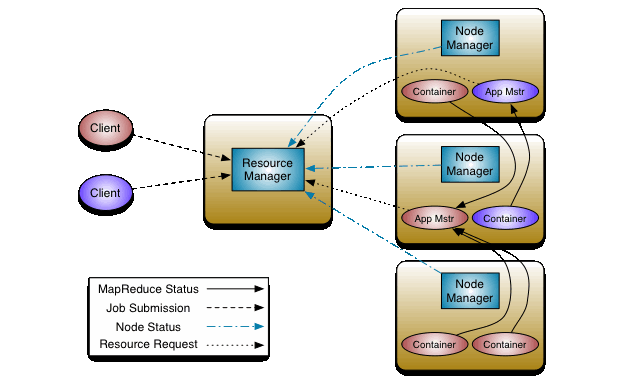
\includegraphics[width=\columnwidth]{./images/yarn_architecture.png}
	\caption[Architektur von YARN]{Architektur von YARN \cite{HadoopYarnDesc272}}
	\label{fig:yarnarch}
\end{figure}

Die Kernidee der Architektur von \textbf{YARN} ist die Trennung vom Ressourcenmanagement und Scheduling. Dazu besitzt der Master den \emph{ResourceManager}, welcher für das gesamte System zuständig ist und die Anwendungen im System überwacht. Er besteht aus zwei Kernkomponenten, dem \emph{ApplicationsManager} und dem \emph{Scheduler}. Der ApplicatonsManager ist für die Annahme und Ausführung von einzelnen Anwendungen zuständig, denen der Scheduler die dafür notwendigen Ressourcen zuteilt und überwacht. Für jeden Slave-\emph{Node} im Hadoop-System gibt es dazu einen \emph{NodeManager}, welcher die lokalen Ressourcen des Nodes überwacht und dem ResourceManager mitteilt. Jede Anwendung besitzt jeweils einen eigenen \emph{ApplicationMaster}, welcher für das Monitoring und die Kommunikation mit dem ResourceManager und NodeManager zuständig ist und die dazu notwendigen Informationen bereit stellt. Jede YARN-Anwendung bzw. Job oder Task besteht zudem aus einem oder mehreren \emph{Containern}, in welchen die Tasks ausgeführt werden. Jeder Bestandteil eines Tasks kann auf jedem beliebigen Node ausgeführt werden \cite{HadoopYarnDesc272}.

\begin{figure}
    \centering
    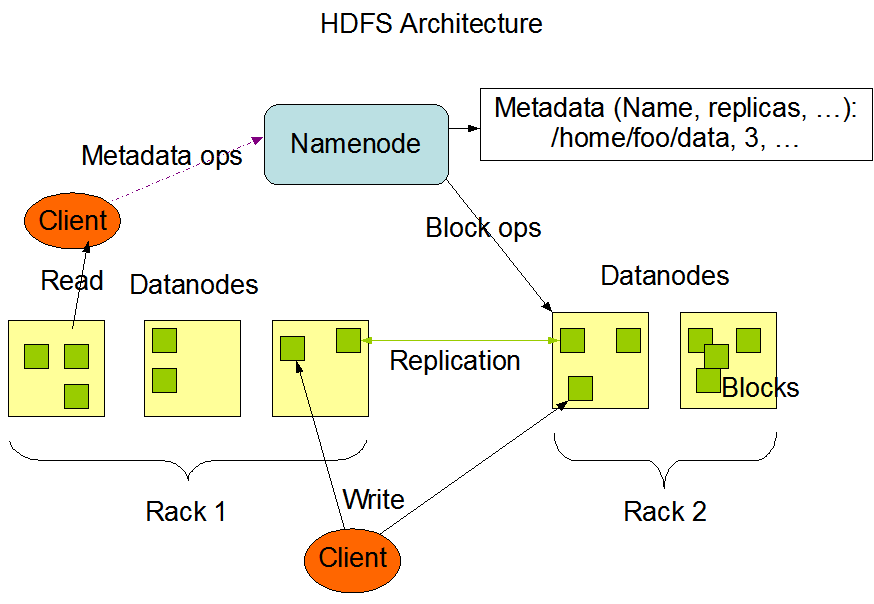
\includegraphics[width=.8\columnwidth]{./images/hdfsarchitecture.png}
    \caption[Architektur des HDFS]{Architektur des HDFS \cite{HadoopHdfsDesc272}}
    \label{fig:hdfsarch}
\end{figure}

Das \textbf{HDFS} basiert auf der gleichen Architektur wie YARN und besitzt ebenfalls einen Master und mehrere Slaves, welches in der Regel die gleichen Nodes sind wie bei YARN sind. Der \emph{NameNode} ist als Master für die Verwaltung des Dateisystems zuständig und reguliert den Zugriff auf die darauf gespeicherten Daten. Die Daten selbst werden in mehrere Blöcke aufgeteilt auf den \emph{DataNodes} gespeichert. Um den Zugriff auf die Daten im Falle eines Node-Ausfalls zu gewährleisten, wird jeder Block auf anderen Nodes repliziert. Dateioperationen (wie Öffnen oder Schließen) werden direkt auf den DataNodes ausgeführt, sie sind darüber hinaus auch dafür verantwortlich, dass Clients die Daten lesen oder beschreiben können \cite{HadoopHdfsDesc272}.

\textbf{MapReduce} bietet analog zu YARN die Möglichkeit, Anwendungen mit einem großen Ressourcenbedarf, welche große Datenmengen verarbeiten, auf einem gesamten Cluster auszuführen. Dazu werden bei einem MapReduce-Job die Eingabedaten aufgeteilt, anschließend von den sog. \emph{Map Tasks} verarbeitet und deren Ausgabe von den sog. \emph{Reduce Tasks} geordnet. Meist wird für die Ein- und Ausgabe der Daten das HDFS genutzt, für die Ausführung der einzelnen Tasks wird YARN genutzt \cite{HadoopMapRedTutorial272}.

%Hier soll Hadoop in einer modifizierten Variante zum Einsatz kommen. In \cite{zhang2016} haben Zhang et. al. eine Verbesserung des Scheduler des ResourceManagers vorgestellt, welche genutzt werden soll. Im Vergleich zur Standard-Einstellung von Hadoop benötigt diese mit einer selbstadaptiven Komponente ausgestatte Modifikation im Schnitt um bis zu 40 Prozent weniger Zeit zur Ausführung eines Tasks. Dazu wird der zur Verfügung stehende Arbeitsspeicher zur Laufzeit so eingeteilt, damit immer die maximal mögliche Anzahl an Tasks ausgeführt werden können.

\onecolumn
% einfacher Zeilenabstand
\singlespacing
% Literaturliste soll im Inhaltsverzeichnis auftauchen
\newpage
\addcontentsline{toc}{chapter}{Literaturverzeichnis}
% Literaturverzeichnis anzeigen
\renewcommand\refname{Literaturverzeichnis}
\bibliography{literatur,abbildungen}

%% Index soll Stichwortverzeichnis heissen
% \newpage
% % Stichwortverzeichnis soll im Inhaltsverzeichnis auftauchen
% \addcontentsline{toc}{section}{Stichwortverzeichnis}
% \renewcommand{\indexname}{Stichwortverzeichnis}
% % Stichwortverzeichnis endgueltig anzeigen
% \printindex

\onehalfspacing
% evtl. Anhang
%\newpage
%\addcontentsline{toc}{section}{Anhang}
%\fancyhead[L]{Anhang} %Kopfzeile links
%%\chapter*{Anhang}\label{chap:anhang}
%\addcontentsline{toc}{chapter}{Anhang}
%\fancyhead[L]{Anhang}
%\renewcommand{\thesection}{\Alph{section}}

\chapter{\glsentryshort{CLI}"=Befehle von Hadoop}
\label{app:hadoopCmds}

Für jede der vier relevanten YARN"=Komponenten können die Daten jeweils als Liste oder als ausführlicher Report ausgegeben werden.
Im Folgenden sind beispielhaft die dafür notwendigen Befehle für Anwendungen aufgelistet, für Attempts, Container und Nodes sind analoge Befehle verfügbar.
Neben den Monitoring"=Befehlen sind auch einige weitere für diese Arbeit relevante Befehle mit ihren Ausgaben aufgelistet.
Die Ausgaben zu den Befehlen sind hier zudem auf das wesentliche gekürzt, \uA da Hadoop bei einigen Befehlen ausgibt, über welche Services (in \cref{lst:hadoopAppListCmd} \zB \gls{TLS}, \gls{RM} und \emph{Application History Server}) die Daten ermittelt werden.
Weiterführende Informationen zu den hier aufgeführten Befehlen sowie die vollständige Befehlsreferenz sind in der Dokumentation von Hadoop \cite{HadoopYarnCmds271} zu finden.

\begin{lstlisting}[label=lst:hadoopAppListCmd,style=plain,
caption={[\glsentryshort{CLI}"=Ausgabe der Anwendungsliste]
    \acrshort{CLI}"=Ausgabe der Anwendungsliste.
    Anwendungen können mithilfe der Optionen \mbox{\texttt{-{}-appTypes}} und \mbox{\texttt{-{}-appStates}} gefiltert werden.}]
$ yarn application --list --appStates ALL
18/02/08 15:37:51 INFO impl.TimelineClientImpl: Timeline service address: http://0.0.0.0:8188/ws/v1/timeline/
18/02/08 15:37:51 INFO client.RMProxy: Connecting to ResourceManager at controller/10.0.0.3:8032
18/02/08 15:37:51 INFO client.AHSProxy: Connecting to Application History server at /0.0.0.0:10200
Total number of applications (application-types: [] and states: [NEW, NEW_SAVING, SUBMITTED, ACCEPTED, RUNNING, FINISHED, FAILED, KILLED]):1
Application-Id	Application-Name	Application-Type	User	Queue	State	Final-State	Progress	Tracking-URL
application_1518100641776_0001	QuasiMonteCarlo	MAPREDUCE	root	default	FINISHED	SUCCEEDED	100%	http://controller:19888/jobhistory/job/job_1518100641776_0001
\end{lstlisting}

\begin{lstlisting}[label=lst:hadoopAppDetailsCmd,style=plain,
caption={[\glsentryshort{CLI}"=Ausgabe des Reports einer Anwendung]
    \acrshort{CLI}"=Ausgabe des Reports einer Anwendung}]
$ yarn application --status application_1518100641776_0001
...
Application Report : 
    Application-Id : application_1518100641776_0001
    Application-Name : QuasiMonteCarlo
    Application-Type : MAPREDUCE
    User : root
    Queue : default
    Start-Time : 1518103712160
    Finish-Time : 1518103799743
    Progress : 100%
    State : FINISHED
    Final-State : SUCCEEDED
    Tracking-URL : http://controller:19888/jobhistory/job/job_1518100641776_0001
    RPC Port : 41309
    AM Host : compute-1
    Aggregate Resource Allocation : 1075936 MB-seconds, 942 vcore-seconds
    Diagnostics :
\end{lstlisting}

\begin{lstlisting}[label=lst:hadoopAppStart,style=plain,
caption={[Starten einer Anwendung in Hadoop"=Benchmark]
    Starten einer Anwendung in Hadoop"=Benchmark.
    Hier mit dem Mapreduce Example \acrlong{pi} und dem Abbruch der Anwendung durch den in \cref{lst:hadoopAppKill} gezeigten Befehl.
    Die Anwendungs"=ID \mbox{\texttt{application\_1520342317799\_0002}} ist hier in Zeile 13 enthalten.}]
$ hadoop-benchmark/benchmarks/hadoop-mapreduce-examples/run.sh pi 20 1000
Number of Maps  = 20
Samples per Map = 1000
Wrote input for Map #0
...
Starting Job
18/03/14 13:06:26 INFO impl.TimelineClientImpl: Timeline service address: http://0.0.0.0:8188/ws/v1/timeline/
18/03/14 13:06:27 INFO client.RMProxy: Connecting to ResourceManager at controller/10.0.0.3:8032
18/03/14 13:06:27 INFO client.AHSProxy: Connecting to Application History server at /0.0.0.0:10200
18/03/14 13:06:27 INFO input.FileInputFormat: Total input paths to process : 20
18/03/14 13:06:27 INFO mapreduce.JobSubmitter: number of splits:20
18/03/14 13:06:27 INFO mapreduce.JobSubmitter: Submitting tokens for job: job_1520342317799_0002
18/03/14 13:06:28 INFO impl.YarnClientImpl: Submitted application application_1520342317799_0002
18/03/14 13:06:28 INFO mapreduce.Job: The url to track the job: http://controller:8088/proxy/application_1520342317799_0002/
18/03/14 13:06:28 INFO mapreduce.Job: Running job: job_1520342317799_0002
18/03/14 13:06:34 INFO mapreduce.Job: Job job_1520342317799_0002 running in uber mode : false
18/03/14 13:06:34 INFO mapreduce.Job:  map 0% reduce 0%
18/03/14 13:06:58 INFO mapreduce.Job:  map 20% reduce 0%
18/03/14 13:06:59 INFO mapreduce.Job:  map 60% reduce 0%
18/03/14 13:07:03 INFO mapreduce.Job:  map 0% reduce 0%
18/03/14 13:07:03 INFO mapreduce.Job: Job job_1520342317799_0002 failed with state KILLED due to: Application killed by user.
18/03/14 13:07:03 INFO mapreduce.Job: Counters: 0
Job Finished in 37.53 seconds
\end{lstlisting}

\begin{lstlisting}[label=lst:hadoopAppKill,style=plain,
caption={[Vorzeitiges Beenden einer Anwendung]
    Vorzeitiges Beenden einer Anwendung.
    Hier wird die in \cref{lst:hadoopAppStart} gestartete Anwendung vorzeitig beendet.}]
$ yarn application -kill application_1520342317799_0002
...
Killing application application_1520342317799_0002
18/03/14 13:07:02 INFO impl.YarnClientImpl: Killed application application_1520342317799_0002
\end{lstlisting}


\chapter{REST"=API von Hadoop}
\label{app:hadoopRestApi}

Wie bei der Ausgabe der Daten der YARN"=Komponenten mithilfe der \gls{CLI} können auch bei der Ausgabe mithilfe der \gls{REST}"=API die Daten als Liste oder als einzelner Report ausgegeben werden.
Der Unterschied zur \gls{CLI} liegt jedoch darin, dass in Listenform und als einzelner Report immer die vollständigen Objekte der Komponenten zurückgegeben werden.
Neben der hier gezeigten und auch in der Fallstudie genutzten Ausgabe im JSON"=Format unterstützt Hadoop auch eine Ausgabe im XML"=Format.
Im Folgenden sind daher beispielhaft die Ausgaben im JSON"=Format für die Anwendungsliste vom \gls{RM} und für Ausführungen vom \gls{TLS} aufgeführt.
Im Rahmen dieser Masterarbeit sind die Rückgaben für Listen von Anwendungen, Attempts, \gls{Container} und der Nodes vom \gls{RM} und bzw. \gls{NM} (Container) sowie des \gls{TLS} (Attempts und Container)relevant.
Weitere Informationen zur \gls{REST}"=API sowie hier nicht gezeigte Pfade für die \gls{YARN}"=Komponenten sind in der Dokumentation in \cite{HadoopYarnTlServer271,HadoopRmApi271,HadoopNmApi271} zu finden.

\begin{lstlisting}[label=lst:hadoopAppListRestRm,style=json,
caption={[REST"=-Ausgabe aller \glspl{Anwendung} vom \acrshort{RM}]
    \gls{REST}"=Ausgabe aller \glspl{Anwendung} vom \acrshort{RM}.
    Die Liste kann mithilfe verschiedener Query"=Parameter gefiltert werden.\\
    URL: \url{http://addr:port/ws/v1/cluster/apps}}]
{
  "apps": {
    "app": [
      {
        "id": "application_1518429920717_0001",
        "user": "root",
        "name": "QuasiMonteCarlo",
        "queue": "default",
        "state": "FINISHED",
        "finalStatus": "SUCCEEDED",
        "progress": 100,
        "trackingUI": "History",
        "trackingUrl": "http://controller:8088/proxy/application_1518429920717_0001/",
        "diagnostics": "",
        "clusterId": 1518429920717,
        "applicationType": "MAPREDUCE",
        "applicationTags": "",
        "startedTime": 1518430260179,
        "finishedTime": 1518430404123,
        "elapsedTime": 143944,
        "amContainerLogs": "http://compute-2:8042/node/containerlogs/container_1518429920717_0001_01_000001/root",
        "amHostHttpAddress": "compute-2:8042",
        "allocatedMB": -1,
        "allocatedVCores": -1,
        "runningContainers": -1,
        "memorySeconds": 1756786,
        "vcoreSeconds": 1546,
        "preemptedResourceMB": 0,
        "preemptedResourceVCores": 0,
        "numNonAMContainerPreempted": 0,
        "numAMContainerPreempted": 0
      }
    ]
  }
}
\end{lstlisting}

\begin{lstlisting}[label=lst:hadoopAttemptListRestTls,style=json,
caption={[REST"=Ausgabe aller Ausführungen einer \gls{Anwendung} vom \acrshort{TLS}]
    \gls{REST}"=Ausgabe aller Ausführungen einer \gls{Anwendung} vom \acrshort{TLS}.\\
    URL: \url{http://addr:port/ws/v1/applicationhistory/apps/{appid}/appattempts}}]
{
  "appAttempt": [
    {
      "appAttemptId": "appattempt_1518429920717_0001_000001",
      "host": "compute-2",
      "rpcPort": 46481,
      "trackingUrl": "http://controller:8088/proxy/application_1518429920717_0001/",
      "originalTrackingUrl": "http://controller:19888/jobhistory/job/job_1518429920717_0001",
      "diagnosticsInfo": "",
      "appAttemptState": "FINISHED",
      "amContainerId": "container_1518429920717_0001_01_000001"
    }
  ]
}
\end{lstlisting}



\end{document}